\documentclass[]{article}
\usepackage{listings} 
\usepackage{graphicx} 
%opening
\title{C++ Directed Graph Library Design Report}
\author{}

\begin{document}

\maketitle

\tableofcontents
\newpage
\section{Introduction}
We present a generic graph library for C++. With this library, user can manage graph structures much more efficiently. Furthermore, our library is easy to use and extend for C++ developers.
\section {Node}
User can define the node type they want to use. In most senarios, a node belongs to a graph. Therefore, in our design, a node is created by declare the graph it belongs to and its information. We use an unique identifier for each node in specific graph. After user call function insert\_node, the function will return back this unique identifier. Afterwards, this handle is used to access the correspoding node.

For simplicity, we do not have a node structure for individual nodes in graph like most previous work. For an individual node, we only have the user-defined type storing informations and the handle assigned by the graph.

The implementation is generic. We use template for different kinds user-defined classes. When user declares a graph, the type of nodes must be defined simultaneously. We use concept to check the input types. A user-defined node type must satify:
\begin{itemize}
	\item
	\end{itemize}

\section {Edge}
In directed graphs, an edge is usually attached with 2 nodes: the from node, and the to node. Therefore, similar to node, an edge is always attached to a specific graph. We use similar structure here. There is no standalone structure for edge. Instead, after user adds an edge to a specific graph, an edge handle including the from node and the to node is returned back.

User can also defined their own types for edges, and such types must satisfy:
\begin{itemize}
	\item 
\end{itemize}

\section{Graph Declarations}
\subsection{General Design}
To our knowledge, the most two common types for graph storage are adjacency matrix and adjacency list. Adjacency matrix is easy to find the edge when we have both ends. However, when the graph is sparse, this storage will introduce much useless space. Adjacency list is better for sparse graphs. Considering this, we divide directed graphs into dense graph and sparse graph.

Furthermore, when we choose containers and algorithms to implement these two structures., to maintain a dynamic node list, we need to keep tracking the validness of those identifiers. The most direct way is to use unordered\_map. However, if the node number is fixed, this extra costs can be avoided. Therefore, we divide the graph into graphs with fixed number of Nodes and graphs with variable number of nodes (for short, fixed graphs and variable graphs).

In this way, we have four different kinds of graphs. We use inheritance to show the relationships (Fig.~\ref{fig:graph}).
\begin{figure}
	\centering
	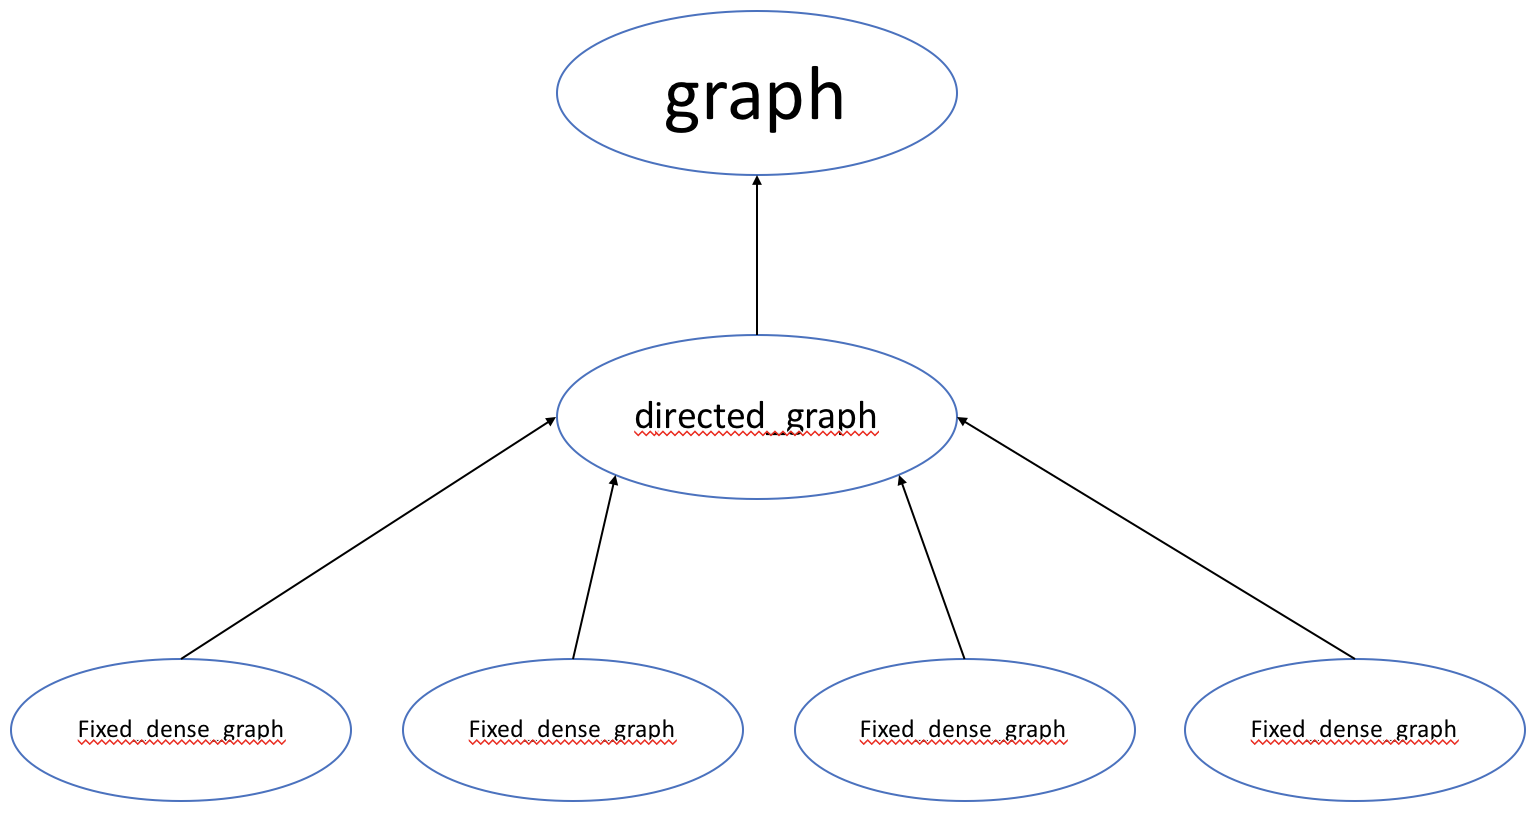
\includegraphics[scale=0.4]{graph.png}
	\caption{Regression Approach Network Architecture}
	
	\label{fig:graph}
\end{figure}
The base graph class is an abstract class. Here we define some fundamental functions for all graphs, including,
\begin{itemize}
	\item
\end{itemize}
The directed\_graph is inherited from base graph class. For now, it does not have any special functions. We put it here is for future inheritance, such as directed acyclic graphs or directed trees.

Next, the four graphs we defined above are all inherited from directed\_graph. Besides implementing the parent class functions, each graph has other special functions based on the underlying data structures. In the following sections, we will show several aspects of each graph's design.
\subsection {Lazy Update Strategy}


\subsection{Graph Maintenance} 
For a general graph, we have several fundamental functions to maintain it.

\subsubsection {Constructor}
The constructor of a graph need to set some variable values and allocate space for the matrix/list.
\subsubsection {Insert Node}
Because we use a unique identifier for each node, the first step to insert a node is to generate this identifier. After that, the node gets pushed into the graph, where we use a vector to save the information of each node. This function returns back this identifier as the handler. The general interface is,
\begin{lstlisting}
node_handle insert_node (V);
\end{lstlisting}
\subsubsection {Insert Edge}
To insert an edge, we need to have the both ends of it and the additional information, so the general interface is,
\begin{lstlisting}
edge_handle insert_edge (node_handle, node_handle, E);
\end{lstlisting}
\subsubsection {Erase Edge}
Erasing an edge is just the reversion of inserting an edge, so the general interface is,
\begin{lstlisting}
void erase_edge (edge_handle);
\end{lstlisting}
\subsection{Graph Visiting}
To implement the graph algorithm, the graph visiting is the most frequency operation. It is necessary for us to design a similar interface for all graph. Visiting a graph includes visiting nodes and visiting edges, and fortunately, there is an approach to design a similar interfaces. 

The answer is to use iterator. No matter to visit all the nodes in a graph or to visit all the out-edges of a node, we need to use for-loop to access each element. It is natural to use an iterator like std::vector. 

Here we implemented the range-for expression. To execute a range-for, all the operations needed are *, != and ++.  In this way, the interface of an iterator is,
\begin{lstlisting}
struct iterator {
	//type members;
	bool operator!=(iterator it) {}
	iterator& operator++() {}
	type operator*() {}
};
\end{lstlisting}
Then, we need to define a container to use this iterator, and the interface of this container is like,
\begin{lstlisting}
struct container {
	iterator begin()const {}
	iterator end()const {}
};
\end{lstlisting}
edge inline
concept
\section{Graph Storage}
\subsection{Dense Graph}
We use adjacency matrix to store graph, because the graph is dense. The element in this matrix is the information of the edge. We use vector to store this structure, so the declaration is,

% 代码环境  
\begin{lstlisting}
vector<vector<E>> adj_matrix;

\end{lstlisting} 
Here the type E is defined by user. 

To mark the validness of each edge, we have another matrix as the flag matrix declared as,
\begin{lstlisting}
vector<vector<bool>> matrix_flag;
\end{lstlisting}

It is intented the dimension of adjacency matrix is fixed when the graph gets constructed. Therefore, the constructor receives a number indicating the max number of the nodes in this graph. Then, it initialze both the adjacency matrix and flag matrix to this fixed dimension by calling push\_back function of std::vector.


For this kind of graph, inserting a node is easy. Firstly, we generate an unique identifier that is the size of node\_vector. Next, we need check if this identifier exceeds the upper bound. If not, we put this node's information into node\_vector.

The argument of function insert\_edge are two node\_handle and the information. What the function does is put this information to corresponding location in adj\_matrix, and set the flag to true.

To erase an edge, we use the late update policy by just setting the flag to false.



\subsection{Sparse Graph}
\subsection{Variable Graph}
\subsection{Fixed Graph}

\section{Path Functions}
\subsection{Generic Path Exists Function}
\subsection{Generic Path Finding Function}

\section{For Developers}

\end{document}
